\documentclass{article}

\usepackage[fleqn]{amsmath} % This package with the fleqn option aligns equations to the left
\setlength{\mathindent}{0pt} % Set indentation from the left margin

\usepackage{amssymb} % Required for math symbols
\usepackage{graphicx} % Required for inserting images
\usepackage{geometry}

\usepackage[backend=biber, style=authoryear, citestyle=authoryear]{biblatex}
\addbibresource{references.bib}

\geometry{a4paper, margin=1in}

{
\title{
    
\includegraphics[width=0.34\textwidth]{/Users/mlnick/documents/images/tsukuba-logo.png} \\
    \vspace{2mm}
    \textbf{Numerical Simulation} \\
    \vspace{3mm}    
    Hometask 2
}

\author{Mamanchuk Mykola, SID.202420671}
% \date{\today}
\date{June 8, 2024}
}

\usepackage{listings}
\usepackage{color}

\definecolor{codegreen}{rgb}{0,0.6,0}
\definecolor{codegray}{rgb}{0.5,0.5,0.5}
\definecolor{codepurple}{rgb}{0.58,0,0.82}
\definecolor{backcolour}{rgb}{0.99,0.99,0.99}

\lstdefinestyle{mystyle}{
    backgroundcolor=\color{backcolour},   
    commentstyle=\color{codegreen},
    keywordstyle=\color{magenta},
    numberstyle=\tiny\color{codegray},
    stringstyle=\color{codepurple},
    basicstyle=\ttfamily\footnotesize,
    breakatwhitespace=false,         
    breaklines=true,                 
    captionpos=b,                    
    keepspaces=true,                 
    numbers=left,                    
    numbersep=5pt,                  
    showspaces=false,                
    showstringspaces=false,
    showtabs=false,                  
    tabsize=2
}
\lstset{style=mystyle}

\begin{document}

\maketitle

\section*{Task 1: Dependence of Fourier Series Coefficients}

The Fourier series for the rectangular and triangular functions decompose these functions into their sinusoidal components, focusing on the coefficients $b_n$ and $a_n$. 

\subsection*{Rectangular Function}
The coefficient $b_n$ for the rectangular function, associated with its sine series due to odd symmetry, is derived as follows:
\[
b_n = \int_0^L f(x) \sin\left(\frac{2\pi nx}{L}\right) dx
\]
For a unit amplitude, this evaluates to:
\[
b_n = \frac{L}{2\pi n} (1 - \cos(\pi n))
\]
This reflects the function's sharp transitions and captures the essence in sine series components.

\setlength{\fboxsep}{0pt} % Removes padding around the image
\setlength{\fboxrule}{0.5pt} % Sets the thickness of the border

% Include the image for bn solution
\begin{figure}[h]
    \centering
    \fbox{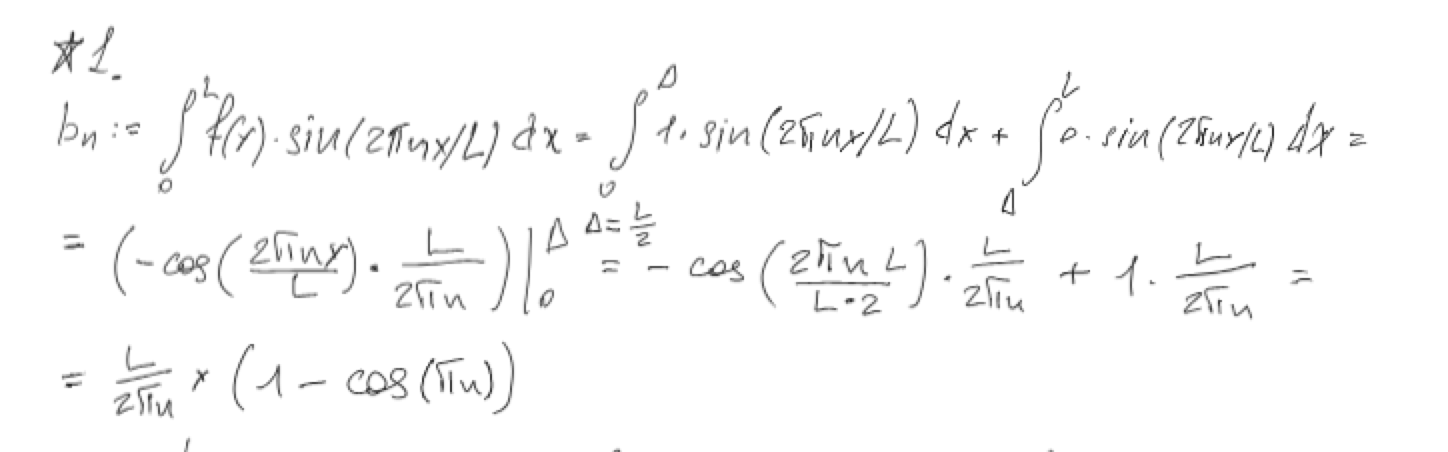
\includegraphics[width=0.8\textwidth]{materials/bn.png}}
    \caption{Solution for \( b_n \)}
    \label{fig:bn_solution}
\end{figure}

\subsection*{Triangular Function}
The coefficients $a_n$ for the triangular function, associated with cosine terms due to even symmetry, are derived as:
\[
a_n = \int_0^L f(x) \cos\left(\frac{2\pi nx}{L}\right) dx
\]
Considering a specific setup:
\[
a_n = \frac{\alpha}{2} \left(\frac{L}{\pi n}\right)^2 (1 + \cos(\pi n))
\]
This captures the linear gradients of the triangular function, smoothing the approximation.

% Include the image for an solution
\begin{figure}[h]
    \centering
    \fbox{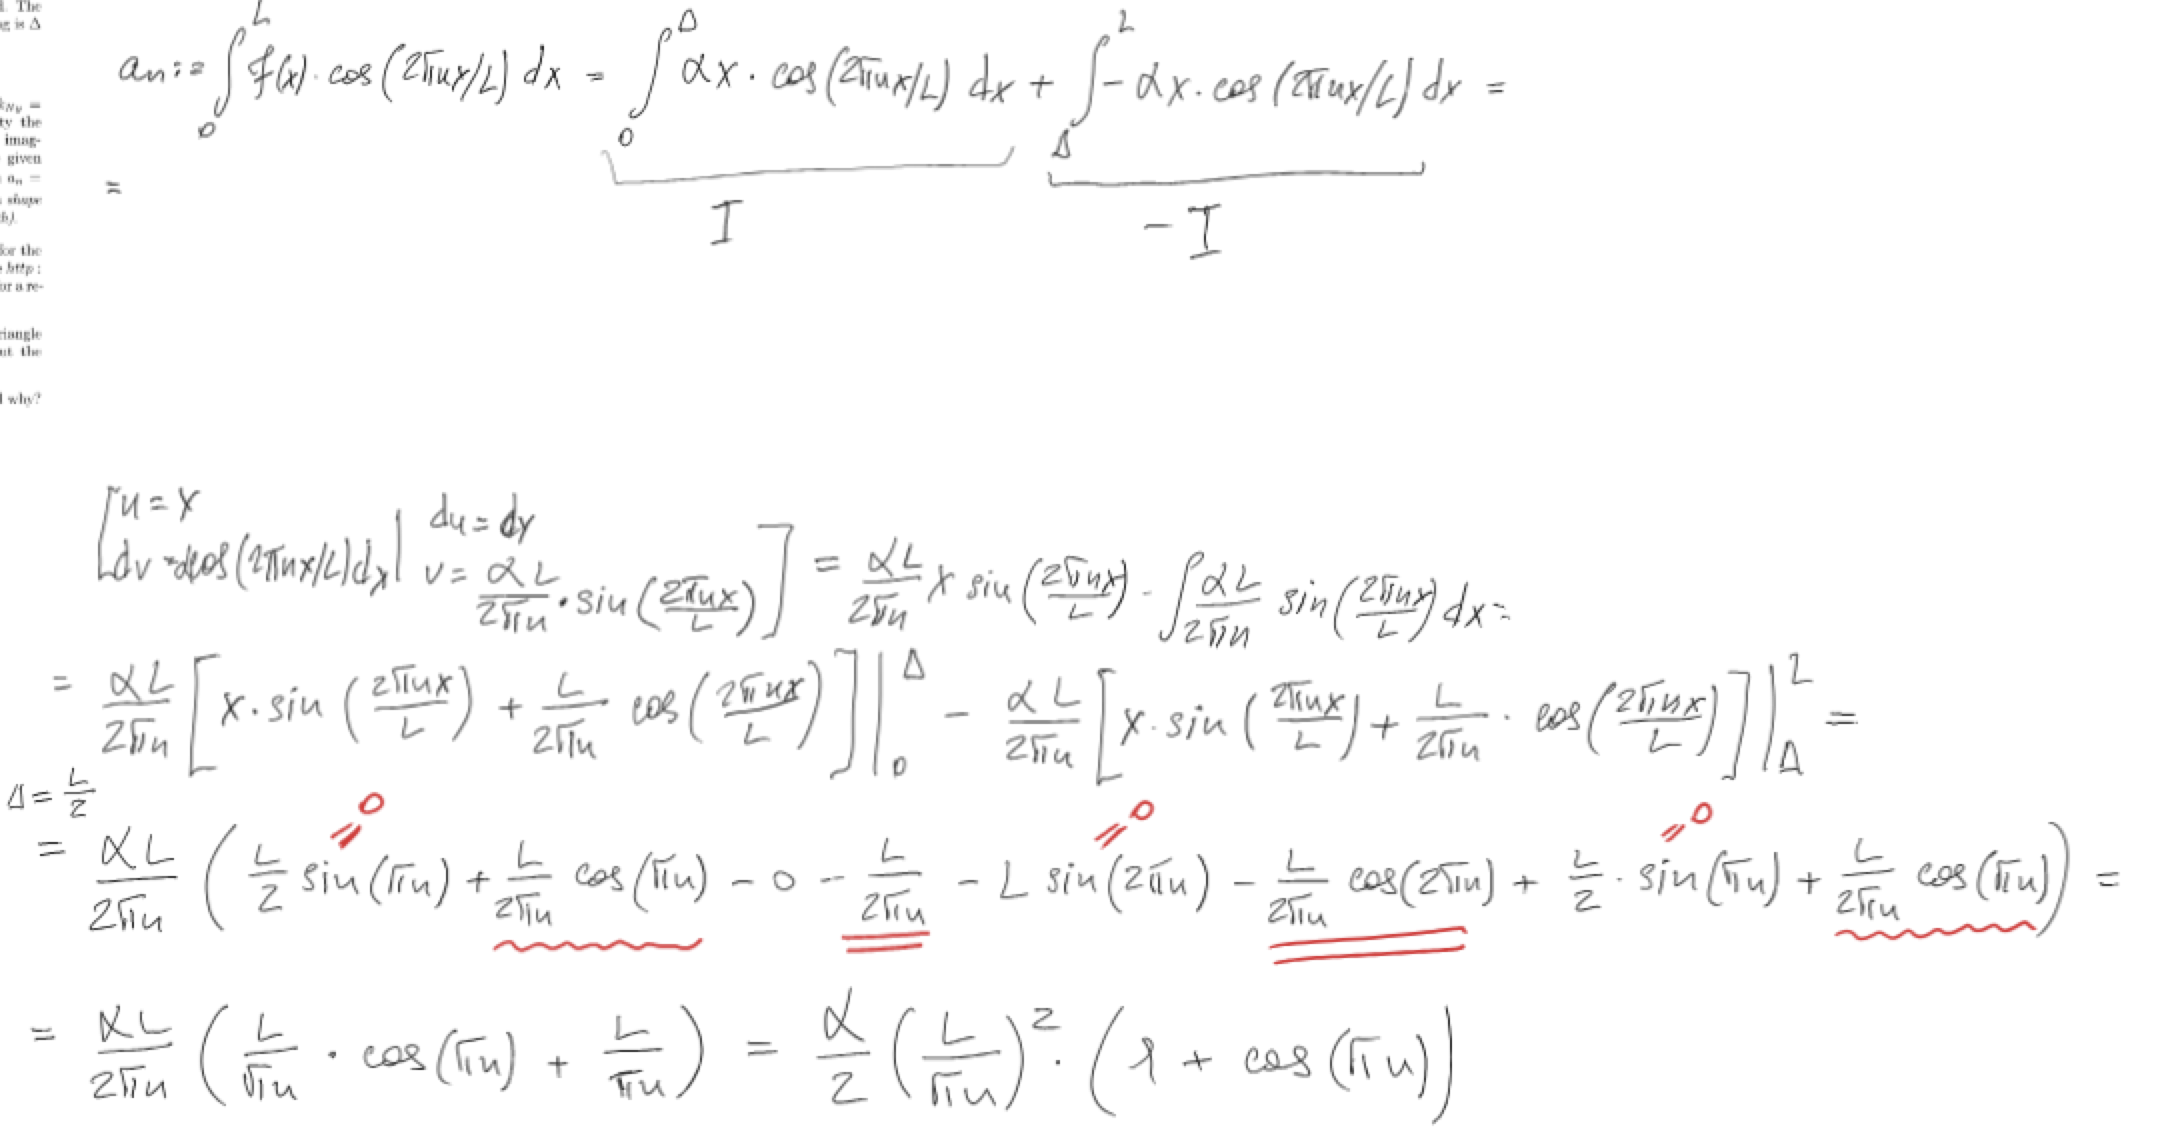
\includegraphics[width=0.8\textwidth]{materials/an.png}}
    \caption{Solution for \( a_n \)}
    \label{fig:an_solution}
\end{figure}

\textbf{Note:}
The variable $n$ represents the harmonic order or frequency component of the Fourier series, enhancing the original function's approximation with more detailed harmonic inclusion.


\section*{Task 2: Further Analysis on Fourier Series}

\subsection*{Alternative Spectrum Computation for Triangular Function}
An interesting alternative to compute the spectrum of the triangular function, given the spectrum of the rectangular function, is through the use of the convolution theorem. In Fourier analysis, convolution in the time domain is equivalent to multiplication in the frequency domain. Since a triangular function can be modeled as the convolution of two rectangular functions, the spectrum of the triangular function can be obtained by squaring the magnitude of the spectrum of the rectangular function:
\[
\hat{f}_{\text{triangle}}(k) = \left(\hat{f}_{\text{rect}}(k)\right)^2
\]
This approach leverages the properties of Fourier transforms to simplify the process and directly relate the characteristics of these fundamental shapes.

\section*{Task 3: Comparative Analysis on Aliasing}
Regarding aliasing effects, using convolution to obtain the spectrum of the triangular function is generally less problematic compared to direct computation. Aliasing, a consequence of insufficient sampling rate, misrepresents high-frequency components as lower frequencies. Through convolution:
\[
\text{Reduced Aliasing} = \text{Effective use of existing data without necessitating higher sampling frequencies}
\]
This method minimizes the risk of aliasing because it inherently smooths the spectrum, spreading the energy of sharp transitions over a broader range of frequencies, thus providing a more faithful representation of the original signal at lower sampling rates.

\vspace{3mm}

\textbf{Note:} The analytical approach through convolution not only simplifies calculations but also provides a more robust method against the aliasing effects commonly encountered in digital signal processing.

\section*{Numerics Exercise 1: Phase Space Distribution Function}

The goal is to analyze a simple Fortran 90 program that simulates an electron plasma within an electrostatic framework. The program includes routines to initialize an electron plasma, compute the charge density, and perform both forward and backward discrete Fourier transforms. These transformations help in understanding the spatial and velocity distributions of electrons.

The phase space distribution function, \( f(x, v_x) \), represents the density of particles in phase space. It is computed using arrays that represent position \( x \) and velocity \( v_x \) of particles. The Fortran code initializes these arrays and then calculates \( f(x, v_x) \) by mapping the distribution of electrons over their respective positions and velocities.

To compare the numerical approximation of \( f(x, v_x) \) with its theoretical or analytical counterpart, plotting both distributions allows for a visual assessment of the accuracy and efficacy of the simulation. This step is crucial for validating the numerical model against known physical behaviors or analytical solutions.

\vspace{3mm}

\textbf{Key Steps in the Simulation:}
\begin{itemize}
    \item Initialize electron plasma with position and velocity arrays.
    \item Compute the phase space distribution function \( f(x, v_x) \).
    \item Plot and compare the numerical results with the analytical function, if available, to verify the simulation's accuracy.
\end{itemize}


\subsection*{Sample Fortran 90 Code for Phase Space Distribution}
\begin{lstlisting}[language=fortran]
program phase_space_distribution
    implicit none
    integer, parameter :: N = 1000
    real, dimension(N) :: x, vx
    real, dimension(N) :: f
    integer :: i

    ! Initialize position and velocity
    do i = 1, N
        x(i) = i * 0.1  ! Example: position spaced at 0.1 units
        vx(i) = sin(real(i) * 0.1)  ! Example: velocity as a function of position
    end do

    ! Compute phase space distribution function
    do i = 1, N
        f(i) = exp(-x(i) * x(i) / 2.0) * exp(-vx(i) * vx(i) / 2.0)  ! Gaussian distribution example
    end do

    ! Output the results (to be plotted externally)
    do i = 1, N
        write(*,*) x(i), vx(i), f(i)
    end do
end program phase_space_distribution
\end{lstlisting}

\newpage

\section*{Numerics Exercise 2: Analyzing DFT Accuracy in Charge Density Computation}

Here we focus on evaluating the accuracy of the Discrete Fourier Transform (DFT) used in computing charge density within a simulation framework. The DFT is advantageous for its ability to handle complex variables efficiently, but it comes with challenges, particularly concerning numerical accuracy and the elegance of the implementation.

\vspace{3mm}

\textbf{Objective:}
\begin{itemize}
    \item Implement both forward and backward discrete Fourier transforms to process charge density.
    \item Analyze the charge density distribution before and after the transforms to evaluate the DFT’s accuracy.
    \item Identify potential sources of error, such as numerical precision issues and the algorithmic handling of complex numbers.
    \item Suggest improvements such as using higher precision arithmetic libraries or optimizing the grid sizes.
\end{itemize}

\textbf{Note:}
Considerations are crucial for understanding how transformations affect the data integrity in simulations and for ensuring that the numerical solutions closely represent the physical phenomena being modeled.

\subsection*{Sample Fortran 90 Code for DFT Analysis}
\begin{lstlisting}[language=fortran]
    program dft_analysis
    implicit none
    integer, parameter :: N = 256  ! Sample size
    complex, dimension(N) :: chargeDensity, dftResult, idftResult
    integer :: i

    ! Initialize the charge density array with some values
    do i = 1, N
        chargeDensity(i) = cos(2.0 * pi * real(i) / real(N)) + sin(2.0 * pi * real(i) / real(N)) * (0.0, 1.0)
    end do

    ! Perform the Discrete Fourier Transform
    call dft(chargeDensity, dftResult, N)

    ! Perform the Inverse Discrete Fourier Transform
    call idft(dftResult, idftResult, N)

    ! Output the results to compare
    do i = 1, N
        write(*,*) 'Original:', chargeDensity(i), 'After IDFT:', idftResult(i)
    end do
end program dft_analysis

subroutine dft(inputArray, outputArray, size)
    complex, dimension(size), intent(in) :: inputArray
    complex, dimension(size), intent(out) :: outputArray
    integer, intent(in) :: size
    integer :: k, n
    complex :: sum

    do k = 1, size
        sum = (0.0, 0.0)
        do n = 1, size
            sum = sum + inputArray(n) * exp(-2.0 * pi * (0.0, 1.0) * real(n - 1) * real(k - 1) / real(size))
        end do
        outputArray(k) = sum / real(size)
    end do
end subroutine dft

subroutine idft(inputArray, outputArray, size)
    complex, dimension(size), intent(in) :: inputArray
    complex, dimension(size), intent(out) :: outputArray
    integer, intent(in) :: size
    integer :: k, n
    complex :: sum

    do k = 1, size
        sum = (0.0, 0.0)
        do n = 1, size
            sum = sum + inputArray(n) * exp(2.0 * pi * (0.0, 1.0) * real(n - 1) * real(k - 1) / real(size))
        end do
        outputArray(k) = sum
    end do
end subroutine idft
\end{lstlisting}

\section*{Numerics Exercise 3: Real Vector Charge Density Handling}

Here all modifications stand for charging density in x-space for a real vector while transforming it into the appropriate subroutines.

\subsection*{Sample Fortran 90 Code for Handling Real Vector Charge Density}
\begin{lstlisting}[language=fortran]
program real_to_complex_dft
    implicit none
    integer, parameter :: N = 256
    real, dimension(N) :: realChargeDensity
    complex, dimension(N) :: complexChargeDensity, dftResult
    integer :: i

    ! Initialize real vector for charge density
    do i = 1, N
        realChargeDensity(i) = sin(2.0 * pi * real(i) / real(N))
    end do

    ! Convert real charge density to complex format for DFT
    do i = 1, N
        complexChargeDensity(i) = cmplx(realChargeDensity(i), 0.0, kind=kind(0.0))
    end do

    ! Call DFT subroutine (to be implemented)
    call dft(complexChargeDensity, dftResult, N)

    ! Output results for verification
    do i = 1, N
        write(*,*) 'DFT Result:', dftResult(i)
    end do
end program real_to_complex_dft

! Sample DFT subroutine (simplified)
subroutine dft(inputArray, outputArray, size)
    complex, dimension(size), intent(in) :: inputArray
    complex, dimension(size), intent(out) :: outputArray
    integer, intent(in) :: size
    integer :: k, n
    complex :: sum

    do k = 1, size
        sum = (0.0, 0.0)
        do n = 1, size
            sum = sum + inputArray(n) * exp(-2.0 * pi * (0.0, 1.0) * real(n - 1) * real(k - 1) / real(size))
        end do
        outputArray(k) = sum / real(size)
    end do
end subroutine dft
\end{lstlisting}

\section*{Numerics Exercise 4: Backward Transform of Electric Field}

This exercise entails computing the electric field by applying the k-space version of the Laplace operator to the transformed charge density. This method replaces the direct computation of the electric field in real space, offering a refined approach to understanding electromagnetic phenomena in simulations.

\vspace{3mm}

\textbf{Methodology:}
\begin{itemize}
    \item The charge density is transformed to k-space using a discrete Fourier transform (DFT).
    \item The electric field in k-space is computed by applying the Laplace operator, which in k-space translates to multiplying by $-k^2$ (where $k$ is the wave number).
    \item An inverse DFT is used to convert the electric field back to real space, allowing observation of the spatial characteristics of the field under different charge density distributions.
\end{itemize}

\textbf{Note:}
This approach is crucial for accurately modeling fields in scenarios where direct real-space calculations may introduce errors or inefficiencies, particularly in homogeneous or near-homogeneous distributions where analytical solutions are complex or intractable.

\subsection*{Sample Fortran 90 Code for Electric Field Computation}
\begin{lstlisting}[language=fortran]
program electric_field_computation
    implicit none
    integer, parameter :: N = 256
    complex, dimension(N) :: chargeDensity, electricField, kSpaceChargeDensity
    real, parameter :: pi = 3.14159265358979323846
    integer :: i

    ! Initialize charge density
    chargeDensity = (1.0, 0.0)

    ! Transform charge density to k-space using DFT
    call dft(chargeDensity, kSpaceChargeDensity, N)

    ! Compute electric field in k-space using Laplace operator
    do i = 1, N
        if (i == 1) then
            electricField(i) = (0.0, 0.0)
        else
            electricField(i) = kSpaceChargeDensity(i) / (-4.0 * pi * pi * (real(i - 1)/real(N))**2)
        endif
    end do

    ! Inverse DFT to get electric field in real space
    call idft(electricField, N)

    ! Output the electric field for visualization
    do i = 1, N
        write(*,*) 'Electric Field:', electricField(i)
    end do
end program electric_field_computation

! Implementations for dft and idft follow...
\end{lstlisting}

\section*{References}
\begin{enumerate}
    \item \textbf{Mamanchuk N., University of Tsukuba}, Github, June 8, 2024. Available online: \url{https://github.com/RIFLE}
    % \item \textbf{Company}, Name of Work, year. Available online: \url{https://...} [Accessed: yyyy-mm-dd]
\end{enumerate}

\end{document}
